\section{Zielsetzung}

In diesem Experiement soll sich der Franck-Hertz-Versuch näher angeschaut werden. Dabei wird die Energiedifferenz zwischen dem ersten angeregten und dem Grundzustand von Hg-Atomen untersucht.
Des Weiteren wird die Ionisationsenergie untersucht.

\section{Theorie}
\label{sec:Theorie}

In dem Franck-Hertz-Versuch werden Elektronenstöße verwendet, um Hg-Atome anzuregen.
Dabei können sowohl elastische als auch unelastische Stöße vorkommen, wobei erstere lediglich die Richtung der Elektronen ändert. 
Der Energieverlust kann hier aufgrund des großen Masseunterschiedes zwischen Hg-Atom und Elektron vernachlässigt werden.
Letztere hingegen sorgen dafür, dass die Elektronen kinetische Energie verlieren. Diese Energie wird zur Anregung des Atoms genutzt.
Die Energiedifferenz der Elektronen ergibt sich damit nach

\begin{equation}
    \label{eqn:e-diff}
    \Delta E = E_1 - E_0 = \frac{m_\text{e}}{2} \cdot (v_\text{vor}^2 - v_\text{nach}^2),
\end{equation}

wobei $m_\text{e}$ die Elektronenmasse und $v_\text{vor}$ und $v_\text{nach}$ die Geschwindigkeiten der Elektronen vor beziehungsweise nach dem unelastischen Stoß sind.
Dies ist ebenfalls die Energie des emittierten Photons, wenn das Atom zurück in den Grundzustand fällt. Dabei gilt die Relation

\begin{equation}
    \label{eqn:photon-energie}
    \Delta E = h \nu
\end{equation}

für die Frequenz $\nu$ des Photons, wobei $h$ das Planck'sche Wirkungsquantum ist.

\begin{figure}
    \centering
    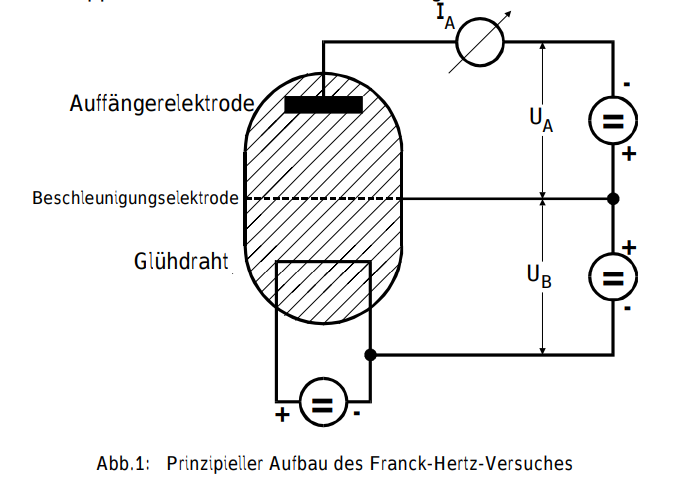
\includegraphics[width=0.8\textwidth]{content/fh-roehre.png}
    \caption{Aufbau einer Röhre mit Gegenfeld\cite{V601}.}
    \label{fig:gegenfeld}
\end{figure}

Zur Bestimmung dieser Energie wird die sogenannte Gegenfeldmethode benutzt.
Hierbei werden die Elektronen in einem Quecksilberdampf mittels einer Beschleunigungselektrode beschleunigt. An dieser liegt die Spannung $U_\text{B}$ an.
Nach dieser befindet sich eine Auffägerelektrode, an der eine Gegenspannung $U_\text{A}$ anliegt. Dieser Aufbau ist in \autoref{fig:gegenfeld} zu sehen.
Wenn die Elektronen auf der Strecke bis zu der Beschleunigungselektrode keine Stöße erfahren und mit der Geschwindigkeit $v = 0$ beginnen, so kann ihre Energie an dieser Stelle mittels

\begin{equation}
    \label{eqn:eU}
    E = e_0 U_\text{B} = \frac{m_\text{e}}{2} v_\text{z}^2
\end{equation}

berechnet werden, wobei $e_0$ die Elementarladung ist.

Wenn diese Geschwindigkeit in $z$-Richtung der Ungleichung

\begin{equation}
    \label{eqn:min-vel}
    \frac{m_\text{e}}{2} v_z^2 \geq e_0 U_\text{A}
\end{equation}

genügt, erreichen die Elektronen die Auffägerelektrode und es kann an dieser ein Strom gemessen werden.
Ist die Beschleunigungsspannung gerade so hoch, dass die Elektronen genug Energie haben, 
um die Hg-Atome anzuregen, so wird man einen starken Abfall der Stromstärke an der Auffängerelektrode feststellen.
Erhöht man die Beschleunigungsspannung weiterhin, so wird dieser Strom erneut ansteigen, 
bis die Elektronen nach dem ersten Anregungsvorgang genug Energie aufnehmen können, um ein weiteres Atom anregen zu können.
In diesem Fall sinkt der Strom an der Auffängerelektrode erneut rapide.
Die dadurch entstehende Theoriekurve ist in \autoref{fig:theo-fh-kurve} zu sehen.

\begin{figure}
    \centering
    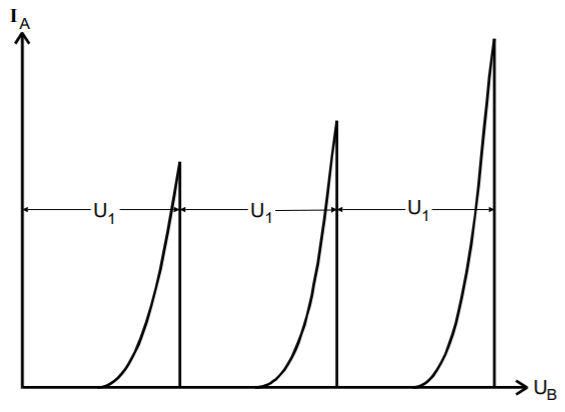
\includegraphics[width=0.8\textwidth]{content/franck-hertz-theorie.PNG}
    \caption{Theoretische Franck-Hertz-Kurve - ohne Störeinflüsse\cite{V601}.}
    \label{fig:theo-fh-kurve}
\end{figure}

Diese Kurve wird in der Praxis allerdings breiter und flacher ausfallen.
Dies liegt daran, dass zum Einen die Elektronen den Glühdraht bereits mit einer gewissen Geschwindigkeitsverteilung verlassen, was dazu führt, dass die Maxima nicht bei einer exakten Spannung festgestellt werden sondern um dieses herum verteilt ebenfalls Stromfluss gemessen wird.
Des Weiteren können die Geschwindigkeitsänderungen durch elastische Stöße zum Teil beträchtlich sein.
Ebenfalls existiert eine gewisse Wahrscheinlichkeit, dass die Elektronen lange genug keinen Stoß erfahren, um das Atom zu ionisieren.
Diese wird möglichst gering gehalten, in dem der Dampfdruck $p_\text{Sättigung}$ in der Röhre auf einem bestimmten Wert gehalten wird. Dadurch entsteht ein bestimmter durchschnittlicher Abstand $\overline{w}$ zwischen den einzelnen Hg-Atomen.
Dieser muss $1000$ bis $4000$ mal kleiner sein als der Abstand $a$ zwischen Glühdraht und Beschleunigungselektrode. Der Abstand zwischen den Atomen und der Sättigungsdruck sind in der Gastheorie miteinander über

\begin{equation}
    \label{eqn:druck-abstand}
    \overline{w} = \frac{0,0029}{p_\text{Sättigung}}
\end{equation}

verknüpft, wobei für die Sättigung mittels

\begin{equation}
    \label{eqn:saettigung}
    p_\text{Sättigung} = 5,5 \cdot 10^7 \cdot e^(\frac{-6876}{T})
\end{equation}

berechnet werden kann. Dabei sind die Einheiten von $\overline{w}$ cm, von $p_\text{Sättigung}$ $10^{-3}$ bar und von $T$ K.


Die Abstände zwischen zwei abrupten Abfällen $U_1$ ist das erste Anregungspotential des Hg-Atoms. Sie berechnet sich über

\begin{equation}
    \label{eqn:anregungspotential}
    U_1 = \frac{1}{e_0} \cdot (E_1 - E_0).
\end{equation}

Des Weiteren ist jedoch zu beachten, dass die Austrittsarbeit des Glühdrahtes und der Beschleunigungselektrode auf den effektiven Wert der Beschleunigungsspannung $U_\text{B,eff}$ miteinwirken.
Diese berechnet sich nach

\begin{equation}
    \label{eqn:accl-eff}
    U_\text{B,eff} = U_\text{B} - \frac{1}{e_0} \cdot (\Phi_\text{B} - \Phi_\text{G}) = U_\text{B} -t K,
\end{equation}

wobei $\Phi_\text{B}$ und $\Phi_G$ die Austrittsarbeit der Beschleunigungselektrode beziehungsweise des Glühdrahtes sind.
Der Summand $\frac{1}{e_0} \cdot (\Phi_\text{B} - \Phi_\text{G})$ wird Kontaktpotential $K$ genannt. Um diesen ist die Franck-Hertz-Kurve verschoben.

\begin{figure}
    \centering
    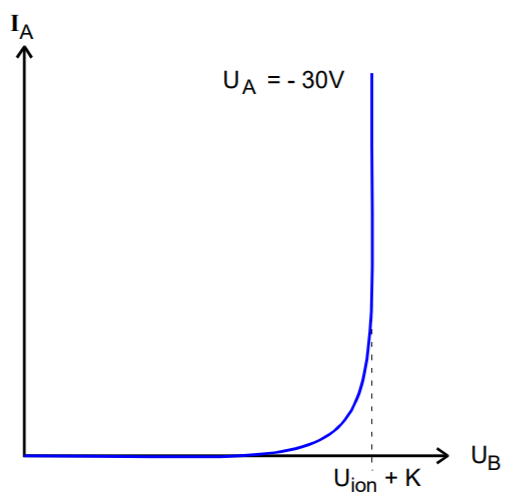
\includegraphics[width=0.6\textwidth]{content/ionisierung.PNG}
    \caption{Theoretische Kurve der Stromstärke $I_\text{A}$ bei dem Ionisationsvorgang\cite{V601}.}
    \label{fig:ion}
\end{figure}

Während der Messung der Ionisationsenergie wird der Wert des Auffängerstroms $I_\text{A}$ zunächst 0 A betragen.
Ist die Ionisationsspannung erreicht, so wird die Stromstärke rapide ansteigen. Die Theoriekurve dazu ist in \autoref{fig:ion} zu sehen.
